\section{Generating Synthetic Controls}

\begin{frame}{Requirements for the Prediction Algorithm}
    \begin{columns}
    \begin{column}{0.5\linewidth}
    \vspace{5pt}
      \begin{enumerate}
         \item {Model non-linear relationships well}
         \item {Robust to unobservables ("heterogeneity-robust") across spatial and temporal dimensions}
         \item {Suitable for high-dimensional space}
      \end{enumerate}
    \end{column}
    \begin{column}{0.5\linewidth}
      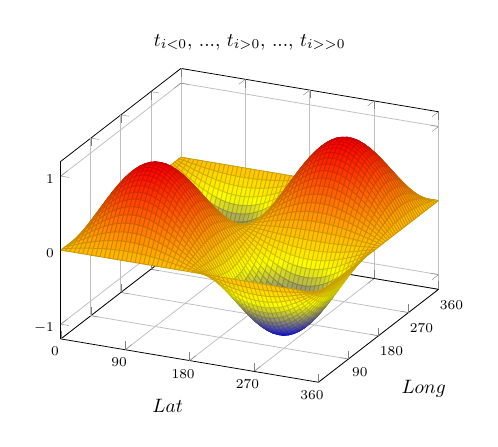
\begin{tikzpicture}[scale=0.70]
      \begin{axis} [
        title = {$t_{i<0}$, ..., $t_{i>0}$, ..., $t_{i>>0}$},
        xtick = {0,90,...,360},
        ytick = {90,180,...,360},
        xlabel = $Lat$, ylabel = $Long$,
        ticklabel style = {font = \scriptsize},
	grid]
        \addplot3 [surf, domain=0:360, samples=60] 
        	{ sin(x)*sin(y) };
        \end{axis}
        \end{tikzpicture}
    \end{column}
  \end{columns}

    \begin{center}
    \vspace{5pt}
    \footnotesize{\textbf{Note}: This problem is currently at the forefront of statistical research. If I had a definitive solution, I would be resting on my laurels right now.}
    \end{center}
\end{frame}

\begin{frame}{Solutions?}

\begin{table}[htbp]
\centering
\begin{tabular}{|p{0.3\linewidth}|p{0.3\linewidth}|p{0.3\linewidth}|}
\hline
\textbf{Machine Learning} & \textbf{Non-Parametric} & \textbf{Dimensionality Reduction} \\
\hline
Strong predictive performance in non-linear relationships & Robust to violations of functional form assumptions & Absorb temporal dimension into fixed effect. \
\hline
\end{tabular}
\end{table}
\end{frame}

\begin{frame}{Inspiration from Literature}

\begin{itemize}
    \item \cite{pouliot2022}
      \begin{itemize}
        \item Krig-and-regress method for spatially misaligned data
        \item Introduces Kriging (prediction) method into spatial econometrics
        \item Relevant discussion on interpolation, aggregation, and spatial filtering techniques
      \end{itemize}
    \vspace{-7pt}
    \item \cite{serraburieletal2020}
      \begin{itemize}
        \item Estimate the effects of wildfires on vegetation
        \item An application of spatial synthetic controls, though treatment is discrete and units are static
        \item Use of Nuclear Norm Matrix Completion Method (see, \cite{athey2021}
      \end{itemize}
  \end{itemize}
\end{frame}

\begin{frame}{My goal}
---
\end{frame}